\documentclass[12pt,a4paper]{article}
\usepackage[utf8]{inputenc}
\usepackage[spanish,es-tabla]{babel}
\usepackage{geometry}
\usepackage{graphicx}
\usepackage{multirow}
\usepackage{tabularx}
\usepackage{mathptmx}
\usepackage{fancyhdr}
\usepackage{array}
\usepackage[table]{xcolor}
\usepackage{titlesec}
\usepackage{setspace}
\usepackage{microtype}
\usepackage{lastpage}
\usepackage{booktabs}
\usepackage{enumitem}
\usepackage{amsmath}
\usepackage{amsfonts}
\usepackage{amssymb}

\graphicspath{{images/}{../images/}{./}}

\geometry{
    top=4.7cm,
    bottom=2.5cm,
    left=2.5cm,
    right=2.5cm,
    headheight=3.9cm,
    headsep=0.4cm
}

\setstretch{1.15}
\setlength{\parindent}{0pt}
\setlength{\parskip}{0.45em}
\setlength{\tabcolsep}{4pt}

\titleformat{\section}
  {\normalfont\fontsize{12}{14.5}\bfseries}{\thesection.}{0.6em}{\uppercase}
\titlespacing*{\section}
  {0pt}{1.8ex plus 0.4ex minus 0.2ex}{0.6ex plus 0.2ex}

\titleformat{\subsection}
  {\normalfont\fontsize{11.5}{13.5}\bfseries}{\thesubsection.}{0.5em}{}
\titlespacing*{\subsection}
  {0pt}{1.4ex plus 0.3ex minus 0.1ex}{0.4ex plus 0.1ex}

\titleformat{\subsubsection}
  {\normalfont\fontsize{10.5}{12.5}\bfseries\itshape}{\thesubsubsection.}{0.4em}{}
\titlespacing*{\subsubsection}
  {0pt}{1.1ex plus 0.2ex minus 0.1ex}{0.3ex plus 0.1ex}

\newcolumntype{Y}{>{\centering\arraybackslash}X}
\newcolumntype{L}{>{\raggedright\arraybackslash}X}
\newcolumntype{C}{>{\centering\arraybackslash}X}

\definecolor{headerblue}{RGB}{26, 54, 93}
\definecolor{darkblue}{RGB}{43, 108, 176}
\definecolor{lightgraybg}{RGB}{248, 248, 248}
\definecolor{tableheader}{RGB}{232, 238, 246}

\newcommand{\docCodigo}{TI-SIGE-ENT-F1-004}
\newcommand{\docVersion}{1.0}
\newcommand{\docProceso}{GESTIÓN DEL ALCANCE / ALINEACIÓN INSTITUCIONAL}
\newcommand{\docElaboracion}{21/08/2026}
\newcommand{\docRevision}{21/08/2026}
\newcommand{\docTitulo}{DEFINICIÓN DEL ALCANCE, RESTRICCIONES Y OBJETIVOS SGC}
\newcommand{\docOrganizacion}{FACULTAD DE INGENIERÍA EN SISTEMAS, ELECTRÓNICA E INDUSTRIAL}
\newcommand{\docSubOrganizacion}{CARRERA DE INGENIERÍA DE SOFTWARE}

\newcommand{\encabezadofrecuente}{%
    \renewcommand{\arraystretch}{1.15}%
    \noindent\makebox[\textwidth][c]{%
    \begin{tabularx}{\textwidth}{|>{\centering\arraybackslash}m{2.8cm}|Y|>{\centering\arraybackslash}m{4.8cm}|}
        \hline
        \multirow{4}{2.8cm}{\centering\raisebox{-1.15cm}{
\includegraphics[width=2.5cm,height=2.0cm,keepaspectratio]{images/logo.png}}}
        & \textbf{\fontsize{9}{11}\selectfont \docOrganizacion} 
        & \textbf{\fontsize{8}{10}\selectfont CÓDIGO:} \fontsize{8}{10}\selectfont \docCodigo \\
        \cline{3-3}
        & \textbf{\fontsize{8.5}{10.5}\selectfont \docSubOrganizacion} 
        & \textbf{\fontsize{8}{10}\selectfont VERSIÓN:} \fontsize{8}{10}\selectfont \docVersion \\
        \cline{2-3}
        & \textbf{\fontsize{8}{10}\selectfont PROCESO:} \fontsize{8}{10}\selectfont \docProceso 
        & \textbf{\fontsize{8}{10}\selectfont ELABORACIÓN:} \fontsize{8}{10}\selectfont \docElaboracion \\
        \cline{2-3}
        & \textbf{\fontsize{8.5}{10.5}\selectfont \docTitulo} 
        & \textbf{\fontsize{8}{10}\selectfont ÚLTIMA REVISIÓN:} \fontsize{8}{10}\selectfont \docRevision \\
        \hline
    \end{tabularx}%
    }%
}

\pagestyle{fancy}
\fancyhf{}
\fancyhead[C]{\encabezadofrecuente}
\fancyfoot[C]{\fontsize{10}{12}\selectfont Página \thepage\ de \pageref{LastPage}}
\renewcommand{\headrulewidth}{0pt}

\begin{document}

\noindent{\fontsize{10.5}{12.5}\selectfont \textbf{Integrantes:} Heidi Villavicencio \quad$\vert$\quad Steeven Toala \quad$\vert$\quad Nixon Hurtado \quad$\vert$\quad Andrea Vásquez}

\vspace{0.25cm}

\section{Título}
\textbf{Denominación del Entregable:} Definición del Alcance, Restricciones y Objetivos SGC -- Código EDT: 1.4

\section{Introducción}
La delimitación formal del alcance del software previene la dispersión del esfuerzo técnico (Scope Creep) y asegura que todos los entregables converjan hacia la modernización de los procesos SGC de la FISEI. En este documento se especifican con precisión los límites del sistema, las integraciones con servicios institucionales, las restricciones técnicas y los objetivos estratégicos formulados bajo criterios SMART.

\section{Objetivo}
\subsection{Objetivo General}
Definir de manera formal las fronteras, restricciones técnicas, supuestos y objetivos SMART del sistema SIGE, garantizando el cumplimiento irrestricto de los formatos SGC de la FISEI.
\subsection{Objetivos Específicos}
\begin{itemize}[leftmargin=1.5em, itemsep=2pt]
    \item Delimitar las funcionalidades formalmente incluidas (In-Scope) y las exclusiones explícitas (Out-of-Scope).
    \item Formular los objetivos SMART del proyecto con metas cuantificables a corto y mediano plazo.
    \item Identificar las restricciones de arquitectura, licenciamiento de software libre y calendarios.
\end{itemize}

\section{Alcance}
\subsection{Límites del Entregable (In-Scope)}
\begin{itemize}[leftmargin=1.5em, itemsep=2pt]
    \item Digitalización integral de los formatos \texttt{UTA-SGC-A-2-1-P7-T1} y \texttt{UTA-SGC-A-2-1-P7-T2}.
    \item Interfaz Web SPA, API Backend RESTful, Base de Datos PostgreSQL 18, MinIO S3 y LanguageTool.
\end{itemize}
\subsection{Exclusiones (Out-of-Scope)}
\begin{itemize}[leftmargin=1.5em, itemsep=2pt]
    \item Módulos de nómina o pagos y control biométrico físico de asistencia docente.
\end{itemize}

\section{Definiciones}
\begin{itemize}[leftmargin=1.5em, itemsep=2pt]
    \item \textbf{Scope Creep:} Expansión incontrolada del alcance de un proyecto sin ajustes en tiempo ni costos.
    \item \textbf{Objetivos SMART:} Objetivos Específicos (Specific), Medibles (Measurable), Alcanzables (Achievable), Relevantes (Relevant) y Temporales (Time-bound).
    \item \textbf{Frontera del Sistema:} Perímetro que define qué responsabilidades residen dentro de la plataforma y cuáles son externas.
\end{itemize}

\section{Responsabilidades}
\begin{itemize}[leftmargin=1.5em, itemsep=2pt]
    \item \textbf{Steeven Toala / Heidi Villavicencio (Responsables EDT 1.4):} Delimitación de fronteras, definición de objetivos SMART y análisis de restricciones.
    \item \textbf{Nixon Hurtado (Backend):} Validación de restricciones de almacenamiento y base de datos.
    \item \textbf{Ing. Paulo Torres (Docente Evaluador):} Aprobación del alcance y límites del proyecto.
\end{itemize}

\section{Normativa Legal y Técnica}
\begin{itemize}[leftmargin=1.5em, itemsep=2pt]
    \item \textbf{Guía PMBOK (7ma Edición):} Gestión del Alcance del Proyecto.
    \item \textbf{Manual de Calidad Institucional UTA:} Sección de Control Operacional de Documentos.
\end{itemize}

\section{Método, Políticas y Contenidos}
Se utilizó análisis de límites y descomposición funcional. En la Figura \ref{fig:s1_04_alcance} se ilustra el esquema de límites y fronteras del sistema.

\begin{figure}[htbp]
    \centering
    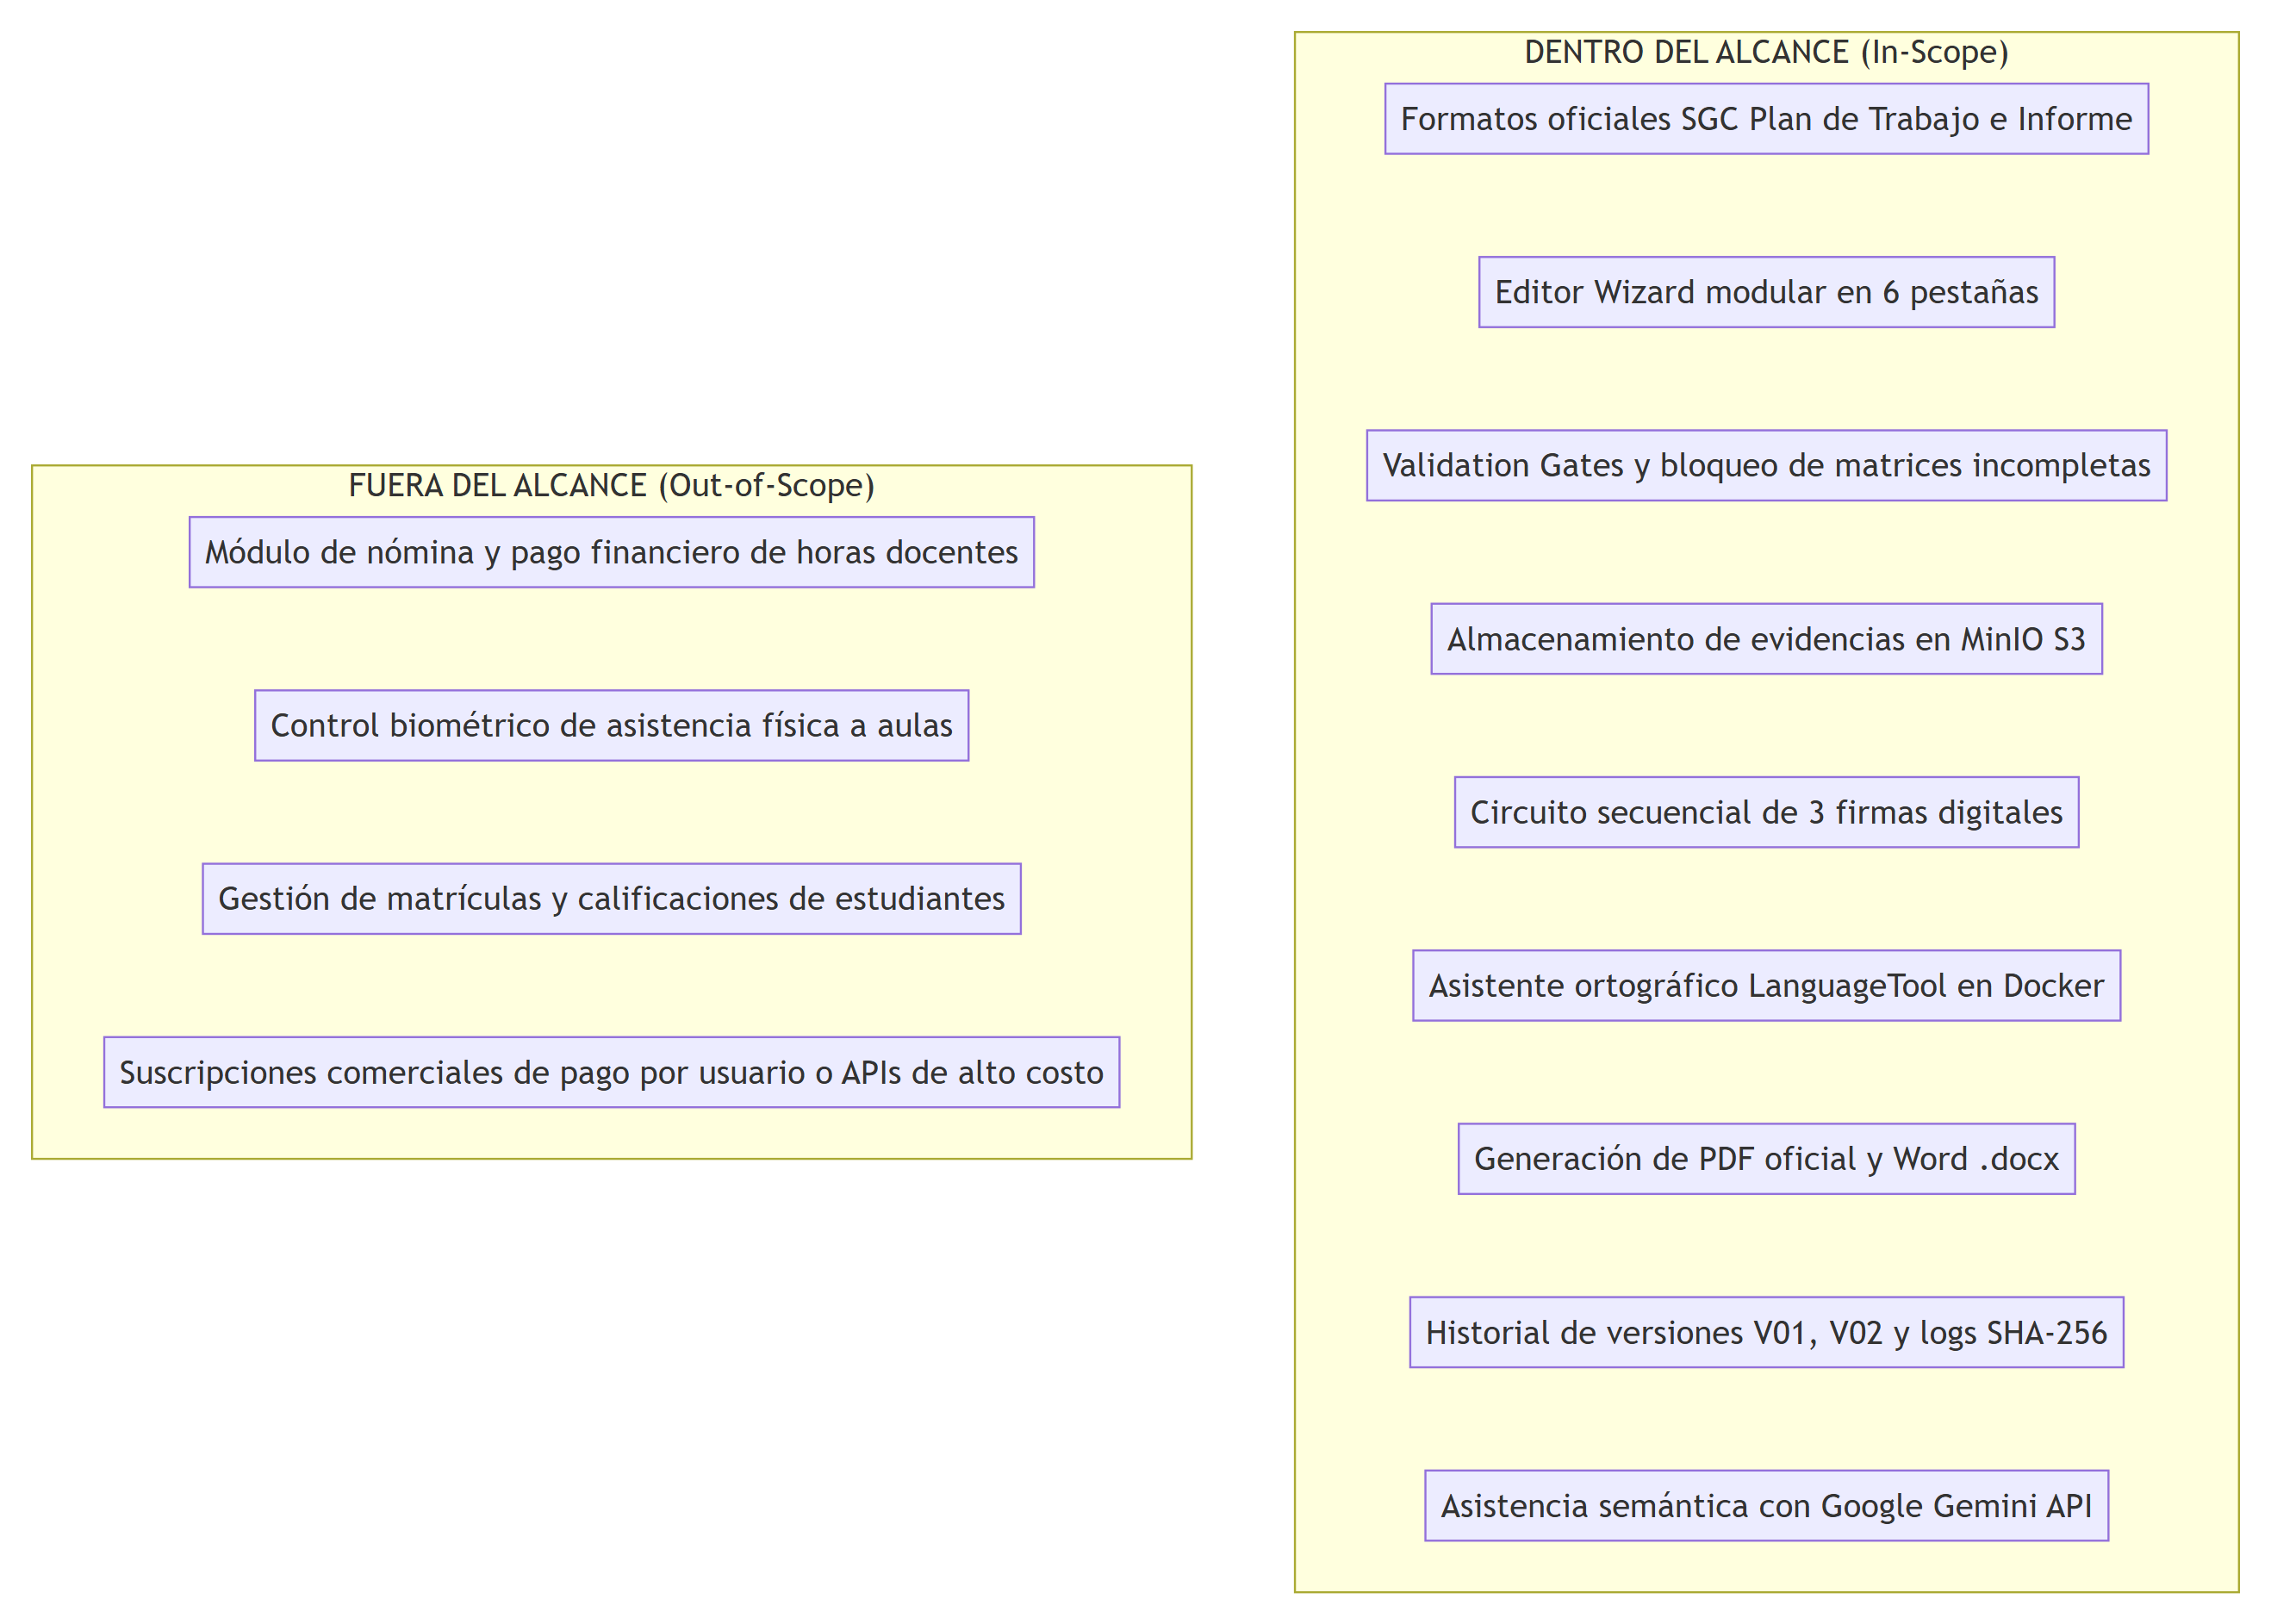
\includegraphics[width=0.88\textwidth,height=5.2cm,keepaspectratio]{images/s1_04_alcance.png}
    \caption{Diagrama de Fronteras y Alcance Operacional del Sistema SIGE.}
    \label{fig:s1_04_alcance}
\end{figure}

\section{Descripción de actividades}
\subsection{Objetivos SMART del Sistema SIGE}
\begin{table}[htbp]
\centering
\small
\renewcommand{\arraystretch}{1.2}
\begin{tabularx}{\textwidth}{|c|>{\bfseries}m{3.2cm}|X|c|}
\hline
\rowcolor{tableheader}
\textbf{No.} & \textbf{Objetivo SMART} & \textbf{Mecanismo de Verificación} & \textbf{Meta} \\
\hline
\textbf{Obj-01} & Reducción de tiempo docente & Medición de tiempo invertido en la elaboración del informe semestral. & Reducir de 8h a 1.5h ($81\%$) \\
\hline
\textbf{Obj-02} & Cero errores aritméticos & Validación estricta por Validation Gate de sumatorias del 100\%. & $0\%$ errores de cálculo \\
\hline
\textbf{Obj-03} & Evidencias auditables & Almacenamiento seguro en MinIO con hash SHA-256 y URLs prefirmadas. & $100\%$ evidencias íntegras \\
\hline
\textbf{Obj-04} & Agilidad en revisiones & Reducción del ciclo de observaciones de coordinadores de área. & De 15 días a 3 días hábiles \\
\hline
\textbf{Obj-05} & Adopción en FISEI & Registro y legalización de informes en la carrera de Software. & $100\%$ docentes involucrados \\
\hline
\end{tabularx}
\caption{Matriz de Objetivos SMART del Proyecto SIGE.}
\label{tab:smart}
\end{table}

\subsection{Restricciones Técnicas y Operativas}
\begin{itemize}[leftmargin=1.5em, itemsep=2pt]
    \item \textbf{Restricción de Infraestructura:} Despliegue completo sobre Docker sin dependencias de licencias propietarias de pago.
    \item \textbf{Restricción de Almacenamiento:} Cuota de 25 MB por archivo adjunto y formatos limitados estrictamente a PDF.
    \item \textbf{Restricción de Formato:} La salida exportada debe mantener idéntica fidelidad tipográfica con los formatos SGC oficiales.
\end{itemize}

\section{Firmas de Responsabilidad}

\noindent
\renewcommand{\arraystretch}{1.2}
\begin{tabularx}{\textwidth}{|>{\raggedright\arraybackslash}m{2.9cm}|>{\raggedright\arraybackslash}X|>{\centering\arraybackslash}m{4.6cm}|>{\centering\arraybackslash}m{2.3cm}|}
    \hline
    \rowcolor{tableheader}
    \textbf{ACCIÓN} & \textbf{NOMBRE Y CARGO} & \textbf{FIRMA} & \textbf{FECHA} \\
    \hline
    \textbf{Elaborado por:} & Heidi Villavicencio\newline Analista de Calidad / UI-UX & \parbox[c]{4.4cm}{\centering\vspace{4pt}
\includegraphics[height=1.5cm,width=4.0cm,keepaspectratio]{images/firma_heidi.png}\vspace{4pt}} & 21/08/2026 \\
    \hline
    \textbf{Revisado por:} & Steeven Toala\newline Líder de Proyecto / Arquitecto & \parbox[c]{4.4cm}{\centering\vspace{4pt}
\includegraphics[height=1.5cm,width=4.0cm,keepaspectratio]{images/firma_steveen.png}\vspace{4pt}} & 21/08/2026 \\
    \hline
    \textbf{Aprobado por:} & Ing. Paulo Torres, Mg.\newline Docente Evaluador -- Gestión Proyectos & \parbox[c]{4.4cm}{\centering\vspace{8pt}\textbf{\textcolor{gray!80}{\scriptsize [ PENDIENTE DE APROBACIÓN ]}}\vspace{8pt}} & \textbf{\textcolor{gray!90}{Pendiente}} \\
    \hline
\end{tabularx}

\vspace{0.4cm}

\section{Control de Cambios}

\noindent
\renewcommand{\arraystretch}{1.2}
\begin{tabularx}{\textwidth}{|>{\hsize=0.45\hsize\centering\arraybackslash}X|>{\hsize=1.55\hsize\raggedright\arraybackslash}X|>{\hsize=1.2\hsize\raggedright\arraybackslash}X|>{\hsize=0.8\hsize\centering\arraybackslash}X|}
    \hline
    \rowcolor{tableheader}
    \textbf{Versión} & \textbf{Descripción del cambio} & \textbf{Responsable del cambio} & \textbf{Fecha de aprobación} \\
    \hline
    1.0 & Emisión inicial del entregable según EDT del Tablero Trello & Equipo de Proyecto SIGE & 21/08/2026 \\
    \hline
\end{tabularx}

\vspace{0.4cm}

\section{Anexos}
\begin{itemize}[leftmargin=1.5em]
\item \textbf{Anexo 1:} Matriz de Criterios de Aceptación del Alcance.
\end{itemize}

\end{document}
